\newpage
\section{Amplitude modulated radio}

\begin{marginfigure}
\begin{center}
\begin{circuitikz}
%\path (2,0) node[above=2pt](ac) {$c(t)=\cos(\omega_c t)$} to [sV] node[pos=0,inner sep=0pt](b){} (2,2);

\draw (2,1) node[above=2pt](b) {$c(t)=\cos(\omega_c t)$}; %to [sV] node[pos=0,inner sep=0pt](b){} (2,2);

\draw (5,3) node[scale=0.8](out){$y(t)=x(t)c(t)$};

\draw (0,3) node[scale=0.8](buf){$x(t)$};

\path (2,2) to [sV,color=white,name=M1] node [midway,above=0.1cm]{Mixer}(2,4);
\mixer{M1}
\draw[ar] (b)--(M1);
\draw[ar] (buf)--(M1);
\draw[ar] (M1)--(out);
\end{circuitikz}
\end{center}
\caption{A simple block diagram representation of an AM radio signal generator system,
which multiplies an audio signal $x(t)$ with a carrier wave $c(t)=\cos(\omega_c t)$.}
\label{fig:am_radio_tx}
\end{marginfigure}

One application of the convolution theorem is explaining how amplitude
modulated (AM) radio works. This is a nice and simple example, but it
also demonstrates a more abstract concept of up- and downconversion of
signals, which is used e.g., in radio hardware\footnote{This same
principle is used by nearly all radio devices, such as the radios
found in your smartphone. The only difference is that the signal
$x(t)$ does not represent an audio waveform, but a scheme that encodes
digital information into a 1d waveform.}.

Upconversion means that a signal is shifted in frequency up to a
higher frequency range. Downconversion means the opposite of that.

The underlying principle behind amplitude modulation is very
simple. An audio signal $x(t)$ is multiplied\footnote{In the early
days of radio, this multiplication was implemented using vacuum
tubes. It can also be implemented using a transistor or a diode
circuit. Nowadays, it is more and more common to modulate signals with
digital signal processing. Mathematically, the operation is the same
for all cases.} with a carrier signal $c(t)=\cos(\omega_c t)$, which
is a high frequency sinusoidal signal:
\begin{align}
y(t) &= x(t)c(t) \\
     &= x(t)\cos(\omega_c t)\,\,.
\end{align}
This is depicted in the block diagram shown in Figure \ref{fig:am_radio_tx}.

Here $\omega_c=2\pi f_c$ is the carrier angular frequency. A typical
carrier frequency $f_c$ for AM terrestrial radio transmissions is
$f_c \in [0.1,30]$ MHz.

These types of radio transmissions that provide global radio
broadcasts still exist. Because signals bounce between the Earth's
ionosphere and ground in this frequency range, signals transmitted
from one location in the world can in optimal conditions travel to the
other side of the Earth.

We'll now study what the spectrum $\hat{y}(\omega)$ of signal $y(t)$
looks like. The key to understanding what $\hat{y}(\omega)$ looks like
is that the spectrum of the signal $x(t)$ is band-limited. This means
that $\hat{x}(\omega) = 0$ when $|\omega|
> \omega_{\mathrm{max}}$. For example, in the case of audio, we know
that there are no audible spectral components at frequencies above 20
kHz. Therefore, in order to transfer an audio signal, we do not need
to include higher frequency components.

In Figure \ref{fig:am_spectra0}, the magnitude spectrum of the real-valued audio
signal $|\hat{x}(\omega)|$ is shown with a red line. The plot
represents a magnitude spectrum for an arbitrary real-valued signal
that occupies angular frequencies between
$\pm \omega_{\mathrm{max}}$. Because the audio signal is real-valued
$x(t)\in \mathbb{R}$, the magnitude spectrum is symmetric around the
y-axis.
\begin{figure}
\begin{center}
\pgfplotsset{
    dirac/.style={
        mark=triangle*,
        mark options={scale=2},
        ycomb,
        scatter,
        visualization depends on={y/abs(y)-1 \as \sign},
        scatter/@pre marker code/.code={\scope[rotate=90*\sign,yshift=-2pt]}
    }
}
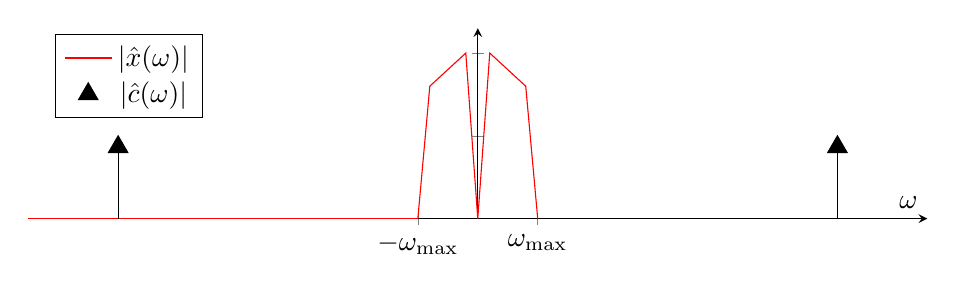
\begin{tikzpicture}
	\begin{axis}[
        width=13cm,
        height=4cm,
        ymin=0,
        ymax=2.3,
    	xmin=-7.5,
        xmax=7.5,
        xlabel={$\omega$},
%        ylabel={$\hat{x}(\omega)$},
        axis x line=center, 
        axis y line=center, 
        yticklabels={,,,},
        xtick={-1,1},
        legend pos=north west,
        xticklabels={$-\omega_{\mathrm{max}}$,$\omega_{\mathrm{max}}$}
    ]
    \addplot[mark=none,color=red] plot coordinates {(-10,0.0) (-1,0) (-0.8,2*0.8) (-0.2,2*1) (0,0) (0.2,2*1) (0.8,2*0.8) (1,0) } ;
\addplot +[dirac,color=black] coordinates {(-6,1.0) (6,1.0)};

%\addplot[mark=none,color=blue] plot coordinates {(-10,0.0) (-7,0) (-6.8,0.8) (-6.2,1) (-6,0) (-5.8,1) (-5.2,0.8) (-5,0) (5,0) (5.2,0.8) (5.8,1) (6,0) (6.2,1) (6.8,0.8) (7,0) (10,0)  } ;
\addlegendentry{$|\hat{x}(\omega)|$}
\addlegendentry{$|\hat{c}(\omega)|$}

%\addlegendentry{$|\hat{Y}(i\omega)|$}
\end{axis}
\end{tikzpicture}
\end{center}
\caption{A spectral representation of signals $x(t)$ and $c(t)$.}
\label{fig:am_spectra0}
\end{figure}
The spectrum of the signal $c(t)$ can be determined by first representing the 
signal as a sum of two complex sinusoids (using Euler's formula):
\begin{equation}
c(t) = \cos(\omega_c t) = \frac{1}{2}e^{i\omega_c t} + \frac{1}{2} e^{-i\omega_c t}\,\,.
\end{equation}
We know that the spectrum of a complex sinusoid is a frequency shifted
Dirac-delta, and hence, the Fourier transform of $c(t)$ is
\begin{equation}
\hat{c}(\omega) = \pi\delta(\omega - \omega_c) + \pi\delta(\omega + \omega_c)\,\,.
\end{equation}
We also know from the convolution theorem, that multiplying two
signals in time domain results in convolution in frequency domain:
\begin{equation}
y(t) = x(t) c(t) \xleftrightarrow{\mathcal{F}} \hat{y}(\omega) = \frac{1}{2\pi}\hat{x}(\omega) * \hat{c}(\omega)\,\,.
\end{equation}
We can now inspect what the spectrum $\hat{y}(\omega)$ looks like by
evaluating the convolution:
\begin{align}
\hat{y}(\omega) & = \frac{1}{2\pi}\int_{-\infty}^{\infty} \hat{x}(\omega') \hat{c}(\omega - \omega') d\omega' \\
  &= \frac{1}{2} \int_{-\infty}^{\infty} \hat{x}(\omega')\left[ \delta(\omega - \omega_c - \omega') + \delta(\omega + \omega_c - \omega') \right] d\omega' \\
   &= \frac{1}{2}\hat{x}(\omega-\omega_c) + \frac{1}{2}\hat{x}(\omega+\omega_c)\,\,.
\end{align}
In this convolution, the Dirac delta functions act as frequency
shifters, which shift the function $\hat{x}(\omega)$ up and down in
frequency by $\omega_c$.

Figure \ref{fig:am_spectra1} shows a plot of the spectrum of the original signal $x(t)$, and the
upconverted signal $y(t)$.
\begin{figure}
\begin{center}
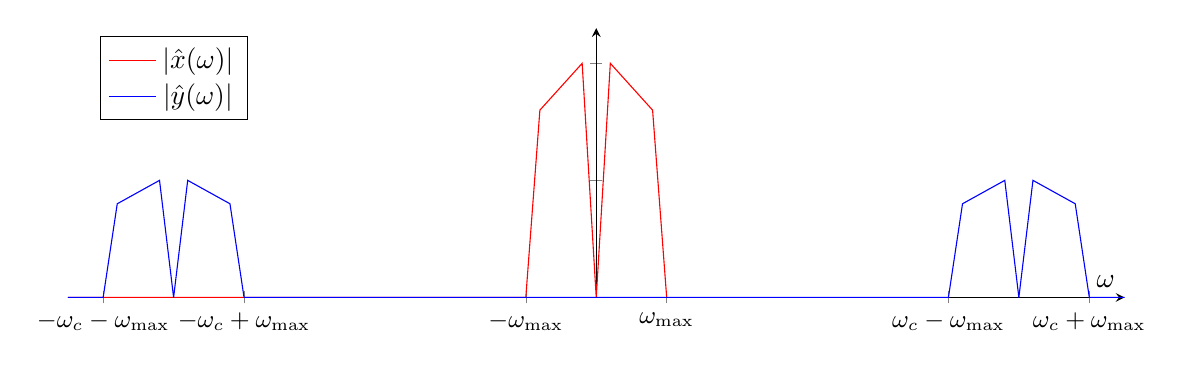
\begin{tikzpicture}
	\begin{axis}[
        width=15cm,height=5cm,ymin=0,ymax=2.3,
    	xmin=-7.5,xmax=7.5,
        xlabel={$\omega$},
%        ylabel={$\hat{Y}(i\omega)$},
        axis x line=center, 
        axis y line=center, 
        yticklabels={,,,},
        ticklabel style = {font=\small},
        xtick={-7,-5,-1,1,5,7},
                legend pos=north west,
        xticklabels={$-\omega_c-\omega_{\mathrm{max}}$,$-\omega_c+\omega_{\mathrm{max}}$,$-\omega_{\mathrm{max}}$,$\omega_{\mathrm{max}}$,$\omega_c-\omega_{\mathrm{max}}$,$ \omega_c+\omega_{\mathrm{max}}$}
    ]
    \addplot[mark=none,color=red] plot coordinates {(-10,0.0) (-1,0) (-0.8,2*0.8) (-0.2,2*1) (0,0) (0.2,2*1) (0.8,2*0.8) (1,0) } ;

\addplot[mark=none,color=blue] plot coordinates {(-10,0.0) (-7,0) (-6.8,0.8) (-6.2,1) (-6,0) (-5.8,1) (-5.2,0.8) (-5,0) (5,0) (5.2,0.8) (5.8,1) (6,0) (6.2,1) (6.8,0.8) (7,0) (10,0)  } ;

\addlegendentry{$|\hat{x}(\omega)|$}
\addlegendentry{$|\hat{y}(\omega)|$}
\end{axis}
\end{tikzpicture}
\end{center}
\caption{The spectrum of the amplitude modulated signal consists of two
copies of the spectrum of the original signal, shifted up and down by
$\omega_c$ in frequency and scaled by $\frac{1}{2}$ in amplitude.}
\label{fig:am_spectra1}
\end{figure}

\newthought{In order to reconstruct the audio signal $x(t)$ from the modulated
signal $y(t)$}, the signal is first multiplied with the carrier
signal:
\begin{equation}
w(t) = y(t)c(t)\,\,.
\end{equation}

This operation again is a frequency shift, just like in the modulation
step. We can again use the convolution theorem to
obtain the spectrum of the intermediate signal $w(t)$:

\begin{marginfigure}[-1.5cm]
\begin{center}
\begin{circuitikz}
%\path (2,0) node[above=2pt]() {$c(t)=\cos(\omega_c t)$} to[sV]node[pos=0,inner sep=0pt](b){} (2,2);

\draw (-2,0) node[](c) {$c(t)=\cos(\omega_c t)$};% to[sV]node[pos=0,inner sep=0pt](b){} (2,2);

\draw (0,-1) node[scale=0.8](bp) {};

\draw (0,-4) node[scale=0.8](out) {$v(t)$};

\draw (0,2) node[scale=0.8](buf){$y(t)=x(t)\cos(\omega_c t)$};

\draw (0.5,-1) node {$w(t)$};

\draw (-0.45,0) node(mixin0){};
\draw (0,0.45) node(mixin1){};

\draw (0,-0.45) node(mixout){};
\draw (0,-1.6) node(bpin){};
\draw (0,-2.4) node(bpout){};

%\path (0,1) to [sV,color=white,name=bp] node[pos=0,inner sep=0pt](d){} node[above left=0.8cm and 0.0cm]{LPF} (0,2);
%\draw (0,2) node(lpf);
%\path (0,0) to [sV,color=white,name=M1] node[midway,above=0.1cm]{Mixer}(0,0);
\draw (0,0) node[inner sep=0pt,color=white] (M1){};
\mixer{M1}
\draw (0,-2) node[sV](bp){};
\LPF{bp}{0}
%\draw[ar] (b)--(M1);
\draw[ar] (c)--(mixin0);
\draw[ar] (buf)--(mixin1);
\draw[ar] (mixout)--(bpin);
\draw[ar] (bpout)--(out);
\end{circuitikz}
\end{center}
\caption{Demodulation or conversion of a high frequency signal $y(t)$ into an audio signal $v(t)$.}
\label{fig:am_demod}
\end{marginfigure}

\begin{align}
\hat{w}(\omega) =& \frac{1}{2\pi} \hat{y}(\omega)*\hat{c}(\omega)\\
 =& \frac{1}{2}\hat{y}(\omega+\omega_c) + \frac{1}{2}\hat{y}(\omega-\omega_c) \\
                 =& \frac{1}{4}\left[\hat{x}(\omega+\omega_c+\omega_c) + \hat{x}(\omega-\omega_c+\omega_c)\right] \\
                 &+ \frac{1}{4}\left[\hat{x}(\omega+\omega_c-\omega_c) + \hat{x}(\omega-\omega_c-\omega_c)\right] \\
                 =& \frac{1}{4}\hat{x}(\omega - 2\omega_c)+ \frac{1}{4}\hat{x}(\omega + 2\omega_c) + \frac{1}{2}\hat{x}(\omega)\,\,.
\end{align}

There are now three copies of the spectrum $\hat{x}(\omega)$. One
centered at $\omega=0$ and two centered at twice the carrier frequency
$\omega=\pm 2\omega_c$ as shown in Figure \ref{fig:am_spectra_demod}.
\begin{figure}
\begin{center}
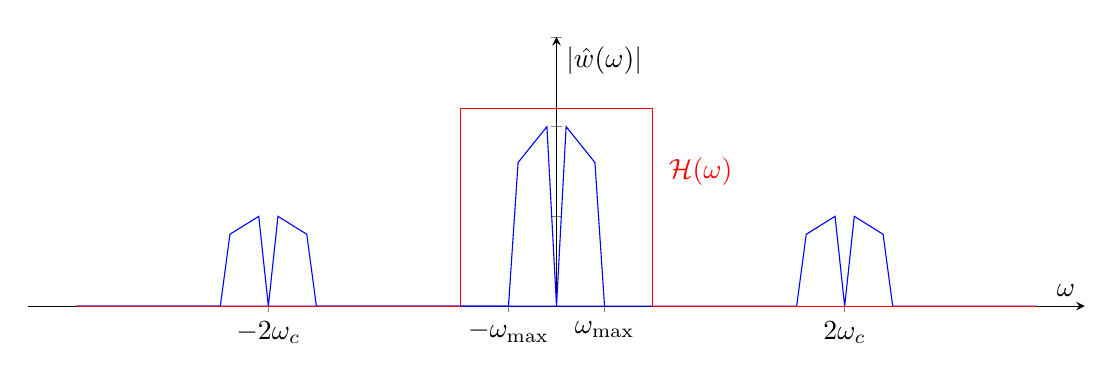
\begin{tikzpicture}
	\begin{axis}[width=15cm,height=5cm,ymin=0,ymax=3,
    	xmin=-11,xmax=11,
        xlabel={$\omega$},
        ylabel={$|\hat{w}(\omega)|$},
        axis x line=center, 
        axis y line=center, 
        yticklabels={,,,},
        xtick={-6,-1,1,6},
        xticklabels={$-2\omega_c$,$-\omega_{\mathrm{max}}$,$\omega_{\mathrm{max}}$,$2\omega_c$}
    ]
    \addplot[mark=none,color=blue] plot coordinates {(-10,0.0) (-1,0) (-0.8,2*0.8) (-0.2,2*1) (0,0) (0.2,2*1) (0.8,2*0.8) (1,0) } ;

\addplot[mark=none,color=blue] plot coordinates {(-10,0.0) (-7,0) (-6.8,0.8) (-6.2,1) (-6,0) (-5.8,1) (-5.2,0.8) (-5,0) (5,0) (5.2,0.8) (5.8,1) (6,0) (6.2,1) (6.8,0.8) (7,0) (10,0)  } ;


\addplot[mark=none,color=red] plot coordinates {(-10,0.0) (-2,0) (-2,2.2) (2,2.2) (2,0) (10,0) } ;

\node at (axis cs:3,1.5) [color=red]{$\mathcal{H}(\omega)$};

%\addlegendentry{$|\hat{w}(i\omega)|$}
\end{axis}
\end{tikzpicture}
\end{center}
\caption{Spectra of an AM demodulated signal.}
\label{fig:am_spectra_demod}
\end{figure}

We almost have what we need, but we need to get rid of the high
frequency components. This can be done with the help of a low-pass
filter:
\begin{equation}
\mathcal{H}(\omega) = \left\{ \begin{array}{cc}
2, & |\omega| \le \omega_{\mathrm{max}} \\
0, & \mathrm{otherwise}
\end{array}\right.\,\,.
\end{equation}
which also corrects the scale back to the original. The frequency
response of such a filter is shown in both Figure \ref{fig:am_spectra_demod} and \ref{fig:am_final_spectrum} with red. The output
signal spectrum is then:
\begin{align}
\hat{v}(\omega) &= \Hiw \hat{w}(\omega) \\
           &= \hat{x}(\omega)\,\,.
\end{align}
And therefore $v(t)=x(t)$. Multiplying with a cosine signal and
low-pass filtering has shifted the signal back to DC and allowed us to
reconstruct the original signal $x(t)$.


\begin{figure}
\begin{center}
\begin{tikzpicture}
	\begin{axis}[width=15cm,height=5cm,ymin=0,ymax=3,
    	xmin=-11,xmax=11,
        xlabel={$\omega$},
        ylabel={$\hat{v}(\omega)=\hat{x}(\omega)$},
        axis x line=center, 
        axis y line=center, 
        yticklabels={,,,},
        xtick={-1,1},
        xticklabels={$-\omega_{\mathrm{max}}$,$\omega_{\mathrm{max}}$}
    ]
    \addplot[mark=none,color=blue] plot coordinates {(-10,0.0) (-1,0) (-0.8,2*0.8) (-0.2,2*1) (0,0) (0.2,2*1) (0.8,2*0.8) (1,0) } ;

%\addplot[mark=none,color=blue] plot coordinates {(-10,0.0) (-7,0) (-6.8,0.8) (-6.2,1) (-6,0) (-5.8,1) (-5.2,0.8) (-5,0) (5,0) (5.2,0.8) (5.8,1) (6,0) (6.2,1) (6.8,0.8) (7,0) (10,0)  } ;


\addplot[mark=none,color=red] plot coordinates {(-10,0.0) (-2,0) (-2,2.2) (2,2.2) (2,0) (10,0) } ;
\node at (axis cs:3,1.5) [color=red]{$\mathcal{H}(\omega)$};

%\addlegendentry{$|\hat{W}(i\omega)|$}
\end{axis}
\end{tikzpicture}
\end{center}
\caption{The original signal spectrum $\hat{x}(\omega)$ reconstructed from the high frequency signal.}
\label{fig:am_final_spectrum}
\end{figure}